\section{Inledning}

\begin{frame}
\frametitle{Ett}
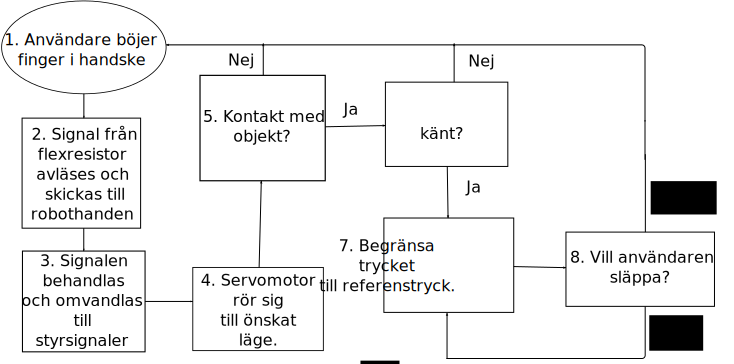
\includegraphics[width=\textwidth]{img/flodesschema}
\end{frame}

\begin{frame}
\frametitle{Ett1}
\includegraphics[width=0.85\textwidth]{img/cutkoskys_handmodeller}
\end{frame}

\section{Robothanden}
\begin{frame}
\includegraphics[width=\textwidth]{img/fingerbild}
\end{frame}
\begin{frame}
\includegraphics[width=\textwidth]{img/stagsenor}
\end{frame}
\begin{frame}
\includegraphics[width=0.5\textwidth]{img/sensor}
\includegraphics[width=0.55\textwidth]{img/trycksensor}
\end{frame}

\section{Styrhandsken}
\begin{frame}
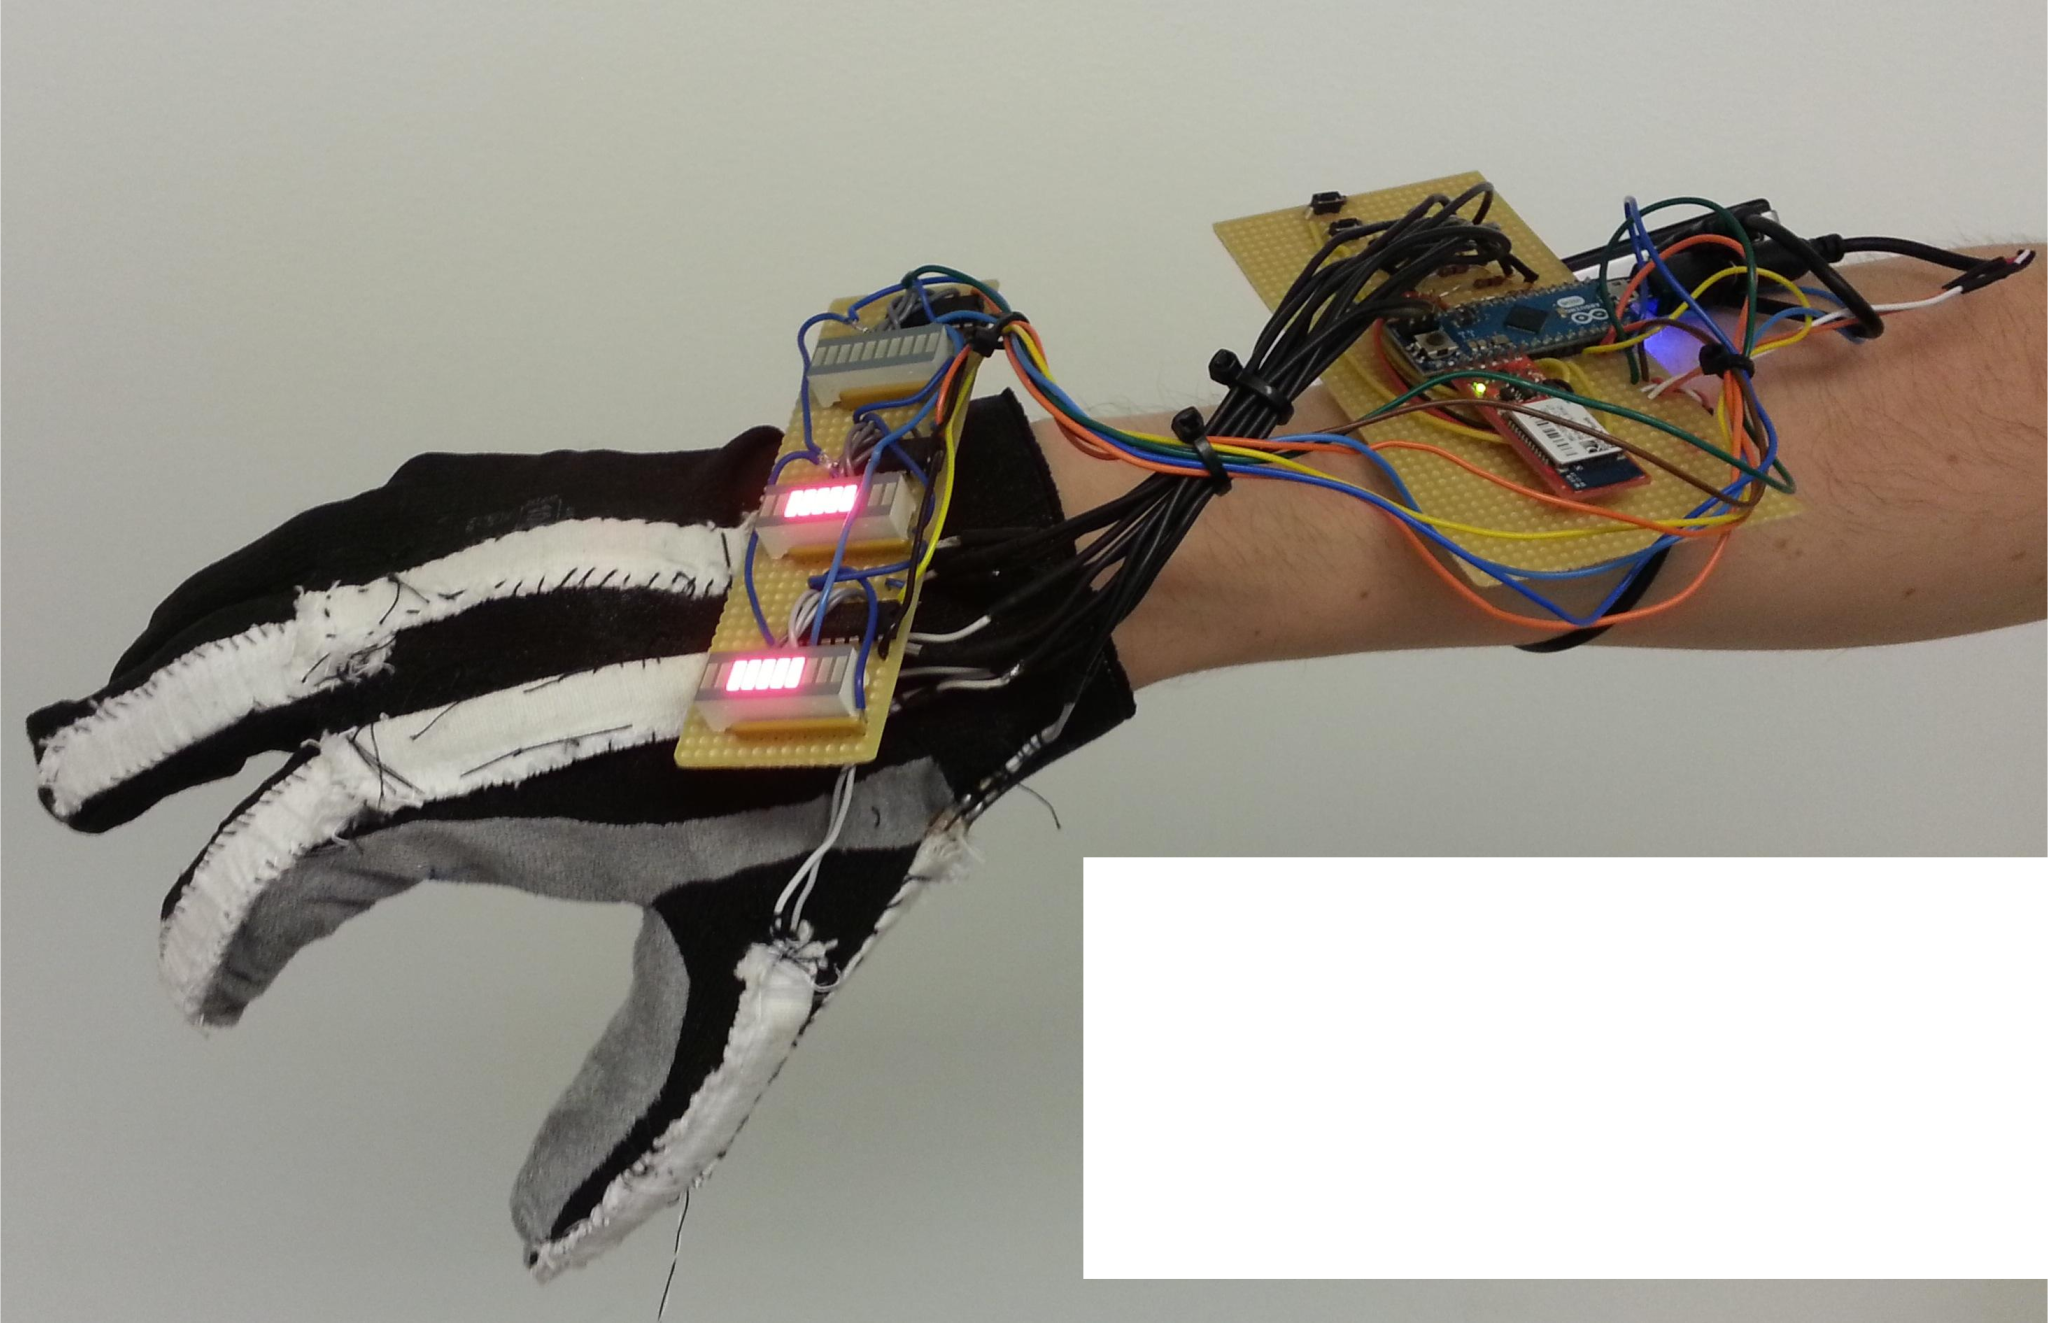
\includegraphics[width=\textwidth]{img/styrhandskediod}
\end{frame}

\section{Signalbehandling}
\subsection{Styrhandsken}
\begin{frame}
\frametitle{Signalens väg för styrhandsken}
\footnotesize
\begin{tikzpicture}[node distance = 2.8cm, auto]
    \node [block] (sampling) {flexsensorernas spänning samplas};
    \node [block, right of=sampling] (filter) {störningar filtreras};
    \node [block, right of=filter] (norm1) {normalisering mot användarens hand};
    \node [block, right of=norm1] (norm2) {normalisering mot robothandens vinklar};

    \path [line] (sampling) -- (filter);
    \path [line] (filter) -- (norm1);
    \path [line] (norm1) -- (norm2);
\end{tikzpicture}
\end{frame}
\subsection{Robothanden}
\begin{frame}
\frametitle{Signalens väg för robothanden}
\begin{tikzpicture}[node distance = 3.5cm, auto]
    \node [block] (sampling) {trycksensorernas spänning samplas};
    \node [block, right of=sampling] (filter) {störningar filtreras};
    \node [block, right of=filter] (norm1) {spänningen räknas om till tryck i Newton};

    \path [line] (sampling) -- (filter);
    \path [line] (filter) -- (norm1);
 \end{tikzpicture}
\end{frame}


\section{Objektidentifiering}
\begin{frame}
\includegraphics[width=\textwidth]{img/servo_vinklar}
\end{frame}
\begin{frame}
\includegraphics[width=\textwidth]{img/matlab_modell}
\end{frame}
\begin{frame}
\includegraphics[width=\textwidth]{img/obj_id_matlab2-eps-converted-to}
\end{frame}

\section{Masterplot}
\begin{frame}
\includegraphics[width=\textwidth]{img/masterplot}
\end{frame}

\section{Diskussion}
\begin{frame}
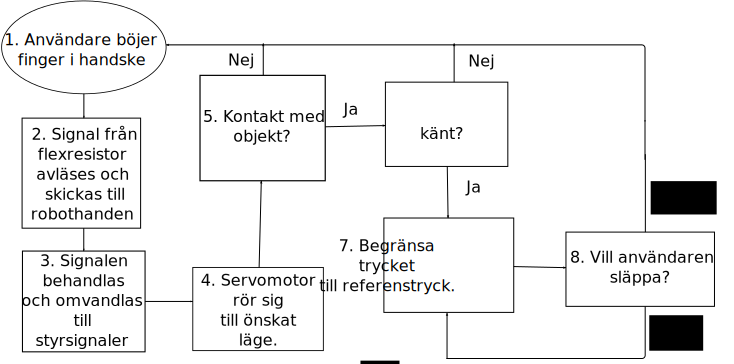
\includegraphics[width=\textwidth]{img/flodesschema}
\end{frame}